\startprefacepage

\textit{Оптимизацией} в математике называется задача нахождения экстремума целевой (оптимизируемой) 
функции в некоторой области конечномерного векторного пространства.

Существует два вида оптимизационных задач:~\cite{wiki_opt}
\begin{enumerate}
\item \textsc{Структурная оптимизация} - задача выбора оптимальной структуры объекта (функции);
\item \textsc{Параметрическая оптимизация} - задача выбора оптимальных числовых значений параметров 
	функции при заданной структуре.
\end{enumerate}

Стандартная математическая задача оптимизации звучит следующим образом. Среди элементов $x$, 
образующих множество $X$, найти такой элемент $x*$, при котором некоторая функция $f(X)$ достигает 
минимального (либо максимального) значения $f(x*)$.

\textit{Многокритериальной оптимизацией} называется процесс одновременной оптимизации нескольких 
конфликтующих целевых функций в некоторой области определения. Задача многокритериальной оптимизации 
состоит в поиске вектора целевых переменных, удовлетворяющего наложенным ограничениям и оптимизирующего 
векторную функцию, элементы которой соответствуют целевым функциям. \cite{wiki_multiopt}
Фактически, задачей многокритериальной оптимизации является одновременное достижение несколькими 
функциями значений, приемлемых для экспериментатора. Критерии оптимальности выбираются в зависимости 
от поставленной задачи.

В данной работе в качестве критерия оптимальности рассматривается \textit{эффективность по Парето}. 
Эффективность по Парето — такое состояние системы, при котором значение каждого частного 
показателя, характеризующего систему (например, каждой из оптимизируемых функций), не может 
быть улучшено без ухудшения по крайней мере одного другого показателя (функции). Множество состояний 
системы, оптимальных по Парето, называется «множеством Парето», или же множеством «неулучшаемых» 
альтернатив.~\cite{wiki_pareto}

	\begin{figure}[h!]
		\center{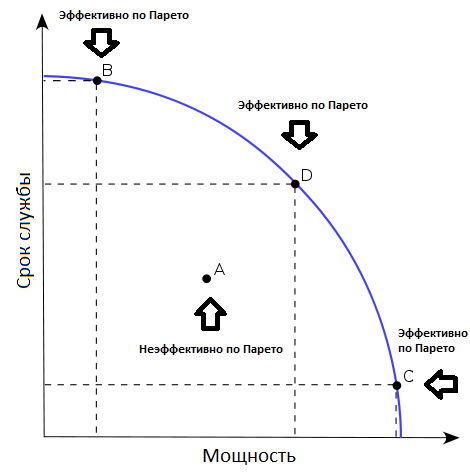
\includegraphics[scale=1]{img/par1}}
		\caption{Пример кривой Парето}
		\label{pict:par1}
	\end{figure}

При решении задачи многокритериальной оптимизации, как правило, используется процедура 
\textit{недоминирующей сортировки}.~\cite{deb_nsga2}
	
Говорят,  что  в K-мерном  пространстве  точка $A = (a_1, ..., a_K)$ доминирует  над  
точкой $B = (b_1,  ..., b_K)$, когда для $1 \le i \le K $ выполняется неравенство 
$a_i \le b_i $ и существует $j$, такое что $a_j < b_j $.

Недоминирующей сортировкой точек в K-мерном пространстве называется процедура, в результате которой:
\begin{itemize}
\item Точки, над которыми не доминирует ни одна точка, помечаются \textit{рангом} 0;
\item Точки, над которыми доминирует хотя бы одна точка ранга 0, помечаются рангом 1;
\item Точки, над которыми доминирует хотя бы одна точка ранга i–1, помечаются рангом i.
\end{itemize}

В результате выполнения недоминирующей сортировки исходное множество точек разбивается на 
\textit{фронты Парето}. Фронтом Парето (или \textit{уровнем недоминирования}) называется 
множество точек, являющихся Парето-оптимальными друг относительно друга. Каждый уровень 
недоминирования характеризуется рангом точек, которые в нем содержатся. Фронт Парето нулевого 
ранга (в случае, если недоминируемые точки помечаются рангом 1~- первого ранга) является множеством 
точек, оптимальных по Парето.

Целью данной работы является разработка структуры данных, поддерживающей корректную 
структуру уровней недоминирования при добавлении новой точки в двумерном пространстве.
В рамках данной работы предложен алгоритм, позволяющий добавлять или удалять точку за 
линейное ($O(N)$, где $N$ - суммарное количество точек на всех уровнях недоминирования)
время. Использование данной структуры данных позволяет, в частности, эффективно реализовать 
инкрементальный алгоритм многокритериальной оптимизации \textit{NSGA-II}. 
\cite{max_me_ss_nsga2}.
